\section{Theorical Foundations}

  \subsection{Fundamentals of Semantic Segmentation}

    \subsubsection{Image Segmentation}

      \ti{Segmentation} is the process of breaking an image into groups of similar
      pixels\cite{intelligence2021modern}, dividing the image into segments. The
      goal of segmentation is to simplify the representation of an image into something
      that is more \ti{meaningful}, allowing more detailed analysis to be performed
      on each segment. There are two ways to approach the problem of segmentation:
      \ti{detecting boundaries} or \ti{detecting regions}\cite{intelligence2021modern}.

      \tb{Boundary detection} involves finding the boundaries between regions, using techniques
      such as edge detection with the Canny algorithm\cite{canny1986computational} or
      thresholding with the Otsu algorithm\cite{otsu1979threshold}. \tb{Region detection}
      involves finding regions of similar pixels, using techniques such as clustering
      with the K-means algorithm\cite{macqueen1965some} or the Mean-Shift algorithm\cite{comaniciu2002mean}.
      Figure \ref{fig:image_segmentation} shows an example of image segmentation using
      both boundary detection and region detection.

      \begin{figure}[htbp]
        \centering
        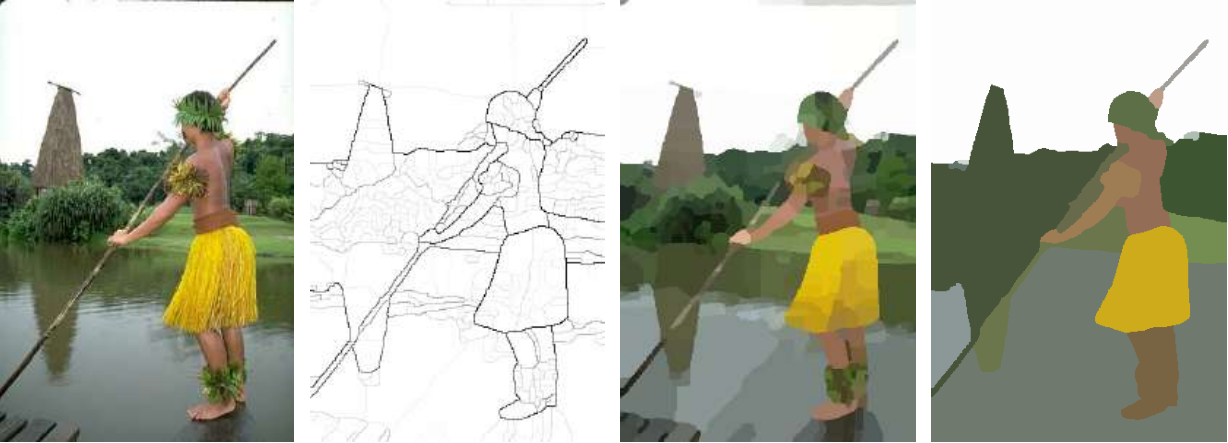
\includegraphics[width=1.00\linewidth]{theorical_foundations/image_segmentation.png}
        \caption{Image Segmentation using boundary and region detection \cite{intelligence2021modern}}
        \label{fig:image_segmentation}
      \end{figure}

    \subsection{Ground Truth}

      \ti{Ground Truth} in the context of semantic segmentation refers to the
      \ti{correct} segmentation of an image, manually annotated as segmentation masks
      that define the boundaries of the objects in the image\cite{intelligence2021modern}.
      The ground truth is used to train, validate and test semantic segmentation models. Pixel-level
      ground truth is the most common type of ground truth used in semantic segmentation
      datasets, where each pixel is assigned a label that defines the object it belongs.
      Figure \ref{fig:cityscapes_semantic_segmentation} and \ref{fig:kitti_semantic_segmentation}
      shows examples of pixel-level ground truth.
 
      \subsubsection{Cityscapes Dataset}

        \ti{Cityscapes} is a dataset for semantic urban scene understanding, containing
        $5000$ high quality pixel-level ground truth images, with $30$ classes of
        objects\cite{cordts2016cityscapes}. Figure \ref{fig:cityscapes_semantic_segmentation}
        shows an example of a Cityscapes image and its corresponding pixel-level ground truth.
        Dataset offers three different splits: \ti{train}, \ti{validation} and \ti{test}.
        As its used for numerous semantic segmentation models, it seems to be the most
        balanced dataset in terms of classes distribution. Also, having some hierarchy
        between classes, it is possible to group them into $8$ upper classes.

        \begin{figure}[htbp]
          \centering
          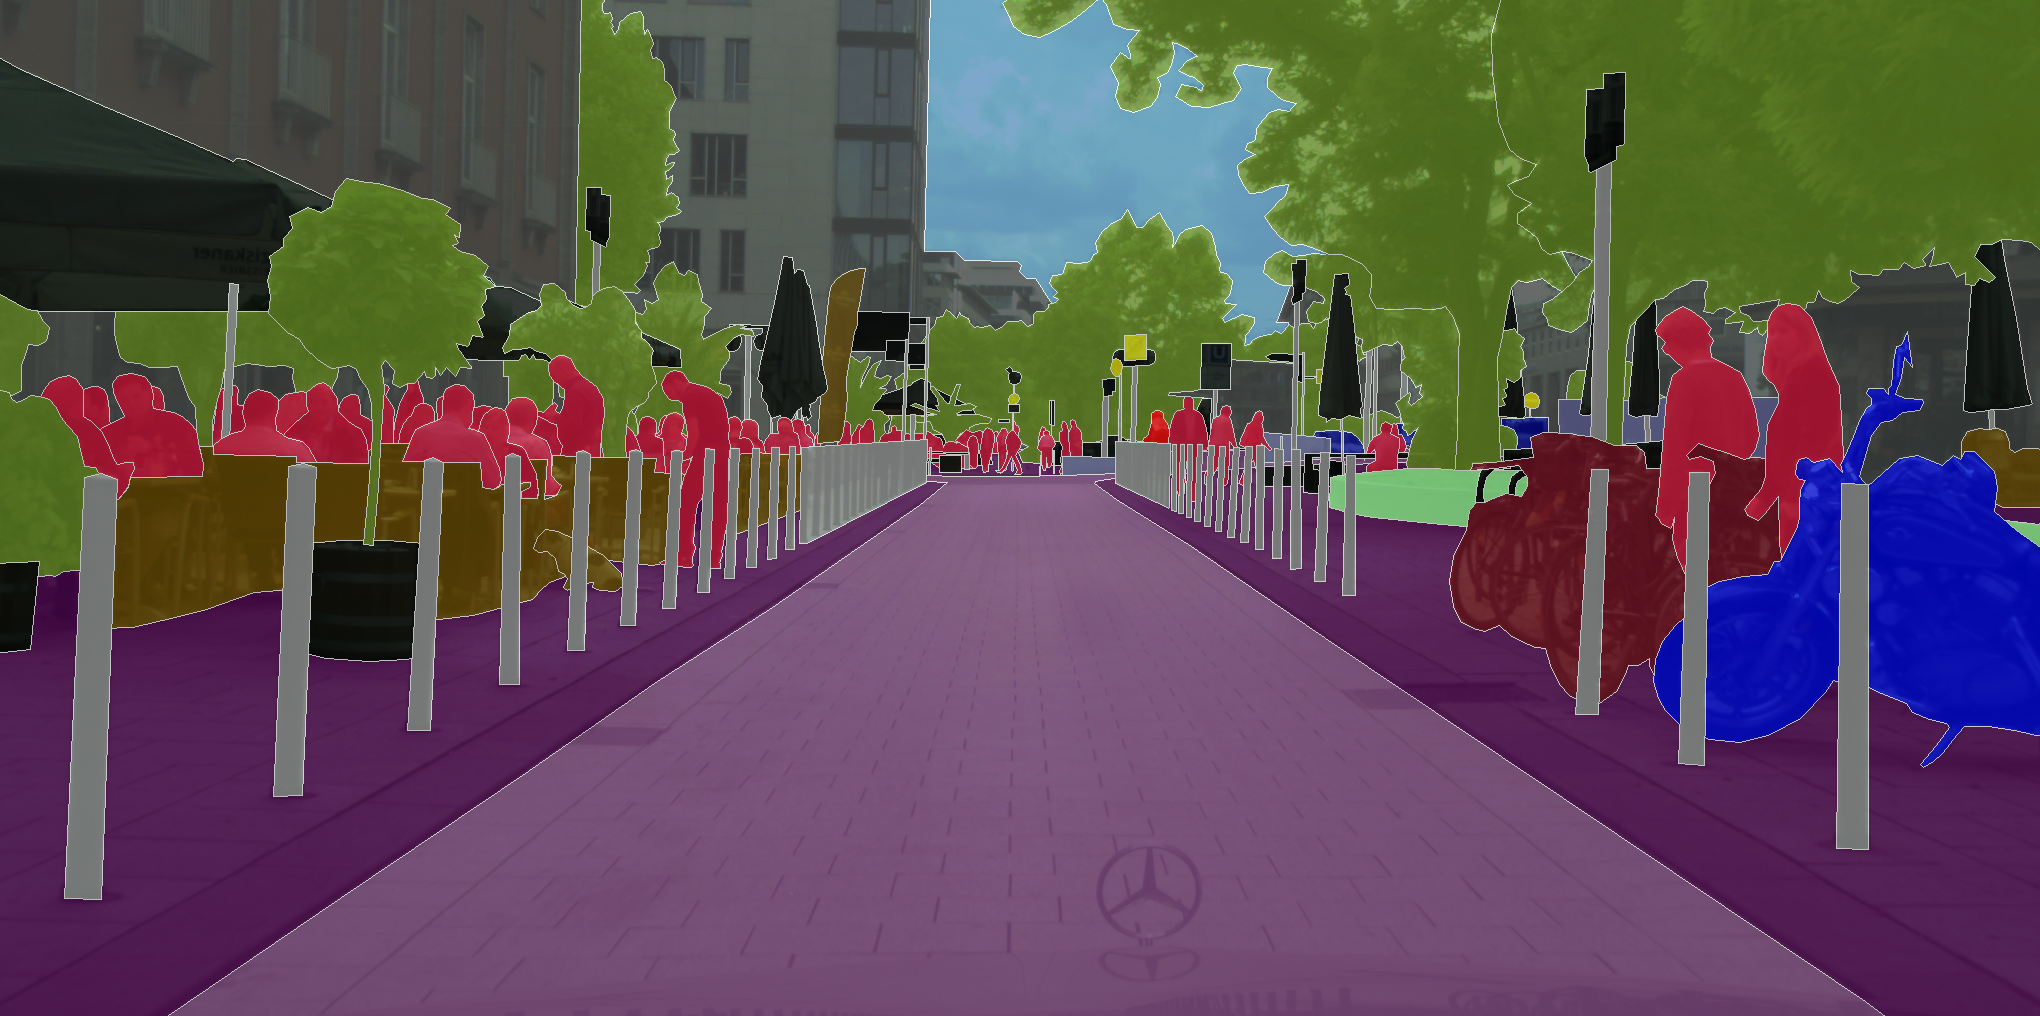
\includegraphics[width=1.00\linewidth]{theorical_foundations/cityscapes_stuttgart.png}
          \caption{Cityscapes semantic segmentation}
          \label{fig:cityscapes_semantic_segmentation}
        \end{figure}

      \subsubsection{KITTI Dataset}

        \ti{KITTI} is a dataset for autonomous driving, containing $200$ pixel-level
        ground truth images, with $34$ classes of objects\cite{Geiger2012CVPR}. Figure
        \ref{fig:kitti_semantic_segmentation} shows an example of a Kitti image and
        its corresponding pixel-level ground truth. Dataset offers two different splits:
        \ti{train} and \ti{test}. As its used for autonomous driving, it seems to be
        the most unbalanced dataset in terms of classes distribution. Also, having no
        hierarchy between classes, it is not possible to group them into upper classes.

        \begin{figure}[htbp]
          \centering
          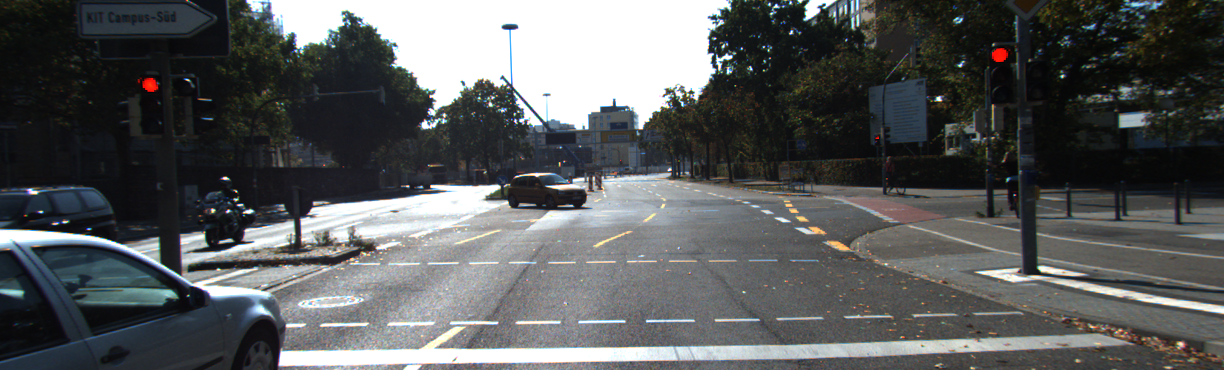
\includegraphics[width=1.00\linewidth]{theorical_foundations/kitti_000155.png}
          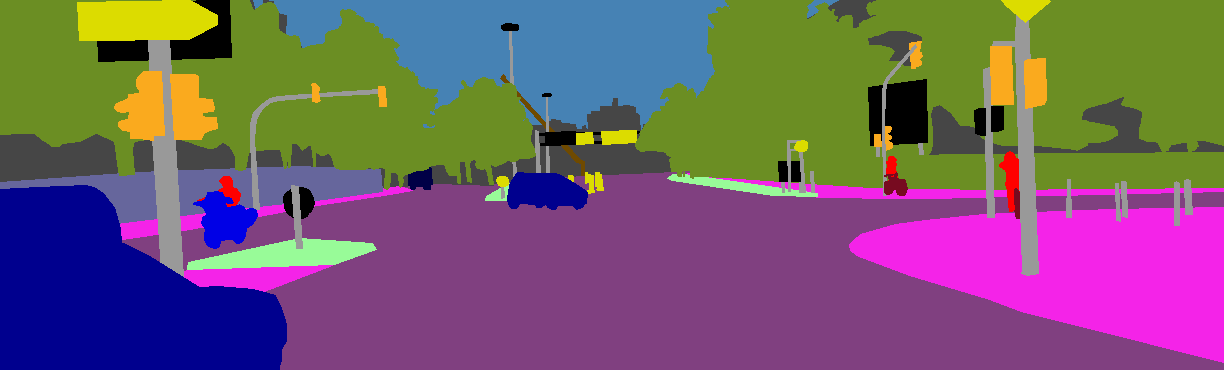
\includegraphics[width=1.00\linewidth]{theorical_foundations/kitti_000155_gt.png}
          \caption{Kitti semantic segmentation}
          \label{fig:kitti_semantic_segmentation}
        \end{figure}

  \subsection{Evaluation Metrics}

    \subsubsection{Pixel Accuracy}

      \ti{Pixel Accuracy (PA)} is the simplest metric used to evaluate the performance
      of a semantic segmentation model. It is calculated by cumputing the ratio
      between the number of correctly classified pixels and the total number of
      pixels in the image\cite{long2015fully}. The pixel accuracy is a value between
      $0$ and $1$, with $1$ being the best possible score.
      \begin{equation}
        \label{eq:pixel_accuracy}
        PA = \frac{TP_i + TN_i}{TP_i + TN_i + FP_i + FN_i}
      \end{equation}
      where $TP_i$ is the number of true positives (correct \ti{foreground pixels}),
      $TN_i$ is the number of true negatives (correct \ti{background pixels})
      meaning correctly classified pixels, $FP_i$ is the number of false positives
      (incorrect \ti{foreground pixels}) and $FN_i$ is the number of false negatives
      (incorrect \ti{background pixels}) meaning incorrectly classified pixels.

      Although the pixel accuracy is a simple metric, it is not a good metric to
      evaluate the performance of a semantic segmentation model. This is because
      the pixel accuracy does not take into account the \ti{class imbalance problem},
      presented in semantic segmentation datasets and real world scenarios.
      
    \subsubsection{Mean Pixel Accuracy}

      \ti{Mean Pixel Accuracy (mPA)} calculate the pixel accuracy(\ti{PA}) for each
      semantic category and then averages the results\cite{long2015fully}. The mPA is a value between $0$ and $1$,
      with $1$ being the best possible score.
      \begin{equation}
        \label{eq:mean_pixel_accuracy}
        mPA = \frac{1}{n} \sum_{i=1}^{n} PA_i
      \end{equation}
      using the same variables as in equation \ref{eq:pixel_accuracy} and $n$ is the
      number of semantic categories. However, the mPA still does not take into account
      the \ti{class imbalance problem}.

    \subsubsection{Intersection over Union}
      
      \ti{Intersection over Union (IoU)} or \ti{Jaccard index} is calculated by dividing
      the intersection of the predicted segmentation and the ground truth segmentation by the union
      of the predicted segmentation and the ground truth segmentation\cite{long2015fully}.
      The IoU is a value between $0$ and $1$, with $1$ being the best possible score.
      \begin{equation}
        \label{eq:iou}
        IoU = \frac{{|A \cap B|}}{{|A \cup B|}} = \frac{TP_i}{TP_i + FP_i + FN_i}
      \end{equation}
      where $A$ is the predicted segmentation, $B$ is the ground truth segmentation,
      $|A \cap B|$ represents the \ti{overlapping area} between $A$ and $B$ meaning
      correctly classified pixels as foreground. While $|A \cup B|$ represents the
      \ti{union area} between $A$ and $B$ meaning all pixels in foreground.

      It is a useful metric to evaluate the performance of a semantic segmentation
      when the \ti{class imbalance problem} is present, take into account the
      presence of small objects and penalize false positives. However, the IoU
      is still not a good metric alone to measure the performance of instance
      segmentation models, because it does not evaluate the background accuracy.

    \subsubsection{Mean Intersection over Union}

      \ti{Mean Intersection over Union (mIoU)} calculate the IoU for each semantic
      category and then averages the results\cite{long2015fully}. The mIoU is a value between $0$ and $1$,
      with $1$ being the best possible score.
      \begin{equation}
        \label{eq:miou}
        mIoU = \frac{1}{n} \sum_{i=1}^{n} IoU_i
      \end{equation}
      using the same variables as in equation \ref{eq:iou} and $n$ is the number of
      semantic categories. The mIoU is a good metric to evaluate the performance of
      a semantic segmentation model, but it still does not evaluate the background
      accuracy.

    \subsubsection{Frecuency Weighted Intersection over Union}

      \ti{Frecuency Weighted Intersection over Union (FWIoU)} extends the mIoU metric
      by taking into account the \ti{class imbalance problem} by assigning a weight
      to each semantic category based on the number of pixels in the ground truth. This
      means that the FWIoU penalizes more the incorrect classification of pixels in
      semantic categories with more pixels in the ground truth, providing a more balanced
      evaluation\cite{lin2017refinenet,long2015fully}. The FWIoU is a value between $0$
      and $1$, with $1$ being the best possible score.
      \begin{equation}
        \label{eq:fwiou}
        FWIoU = \frac{1}{\sum_{i=1}^{n} |B_i|} \sum_{i=1}^{n} |B_i| IoU_i
      \end{equation}
      where $|B_i|$ is the number of pixels in the ground truth for the semantic
      category $i$ (\ti{frequency}) and $n$ is the number of semantic categories.

  \subsection{Fundamentals of Convolutional Neural Networks}

    \Blindtext[1]

    \subsubsection{Convolutions}

      \Blindtext[1]

    \subsubsection{Pooling}

      \Blindtext[1]

    \subsubsection{Fully Connected Layers}

      \Blindtext[1]

    \subsubsection{Skip Connections}

      \Blindtext[1]

    \subsubsection{Activation Functions}

      \Blindtext[1]
  
  \subsection{Fundamentals of Transformers}

    \Blindtext[1]

    \subsubsection{Backbone}

      \Blindtext[1]

    \subsubsection{Encoder}

      \Blindtext[1]

    \subsubsection{Decoder}

      \Blindtext[1]
